\documentclass[11pt]{article}
%Gummi|061|=)
\usepackage{amsmath}
\usepackage{amsthm}
\usepackage{amsbsy}
\usepackage{amssymb}
\usepackage{inputenc}
\usepackage{graphicx}
\usepackage{selinput}
\SelectInputMappings{%
adieresis={ä},
germandbls={ß},
}
\title{\textbf{Versuch V204: Wärmeleitung von Metallen}}
\author{Martin Bieker\\
		Julian Surmann\\
		\\
		Durchgef\"{u}hrt am 31.10.2013\\
		Tu Dortmund}
\date{}
\usepackage{graphicx}
\begin{document}
\renewcommand\tablename{Tabelle}
\renewcommand\figurename{Abbildung}
\maketitle
\thispagestyle{empty}
\newpage
\clearpage
\setcounter{page}{1}


\section{Einleitung}
Im folgenden Versuch geht es um die Untersuchung von Wärmeleitung. Unter Wärmeleitung versteht man den Fluss von Wärme in Richtung geringerer Temparatur. Es wird die Wärmeleitung von mehreren Metallen untersucht. 
\section{Theorie}
Für die Untersuchung des Wärmetransportes in Metallen wird hier nur die Wärmeleitung betrachtet, Konvektion und Wärmestrahlung sind vernachlässigbar.
Die Wärmemenge, die in einer Zeit dt durch die Querschnittsfläche A des zu untersuchenden Stabes fließt, ist gegeben durch:
\begin{equation}
dQ = -\kappa A \frac{\partial T}{\partial x} dt.
\end{equation}
Die Wärmestromdichte $j_w$ ist dann gegeben mit
\begin{equation}
j_w = -\kappa \frac{\partial T}{\partial x}.
\end{equation}
Aus Formel (2) und der Kontinuitätsbedingung lässt sich eine eindimensionale Wärmeleitungsgleichung herleiten:
\begin{equation}
\frac{\partial T}{\partial t} = \frac{\kappa}{\rho c} \frac{\partial^2 T}{\partial x^2}.
\end{equation}
Diese Gleichung gibt die zeitliche und räumliche Entwicklung der Temparaturverteilung an. $c$ steht hier für die spezifische Wärme des Metalles, $\rho$ für dessen Dichte.
$\sigma_T = \frac{\kappa}{\rho c}$ steht damit für die Temparaturleitfähigkeit des Materials. Die Temparaturleitfähigkeit ist ein Maß für Geschwindigkeit, mit der Temparaturdifferenzen neutralisiert werden.
Im zweiten Versuchsteil soll das Ende verschiedener Metallstäbe periodisch erwärmt und gekühlt werden. Dabei entsteht eine räumliche und zeitliche Temparaturwelle. Diese hat die Form
\begin{equation}
T(x,t) = T_{max} e^{\sqrt{\frac{w \rho c}{2 \kappa}}x}cos \left( wt- \sqrt{\frac{w \rho c}{2 \kappa}}x \right).
\end{equation}
Die Phasengeschwindigkeit der Welle ist gegeben mit
\begin{equation}
v = \frac{w}{k} = \frac{w}{\sqrt{\frac{w \rho c}{2 \kappa}}} = \sqrt{\frac{2 \kappa w}{\rho c}}
\end{equation}
Mithilfe der Dämpfung, die aus dem Verhältnis $\frac{A_{nah}}{A_fern}$ folgt, und der Ausdrücke $w = \frac{2 \pi}{T^*}$ ($T^*$ steht für die Periodendauer, nicht für eine Temparatur) und $\Phi = 2 \pi \frac{\Delta t}{T^*}$ folgt für die Wärmeleitfähigkeit
\begin{equation}
\kappa = \frac{\rho c (\Delta x)^2}{2 \Delta t ln(\frac{A_{nah}}{A_{fern}})}
\end{equation}
Hierbei beschreibt $\Delta x$ den Abstand zwischen den beiden Temparaturmessstellen und $\Delta t$ die Phasendifferenz der Wärmewelle zwischen den beiden Messstellen.
\section{Aufbau und Durchf\"{u}hrung}
\begin{figure}[htp]
\centering
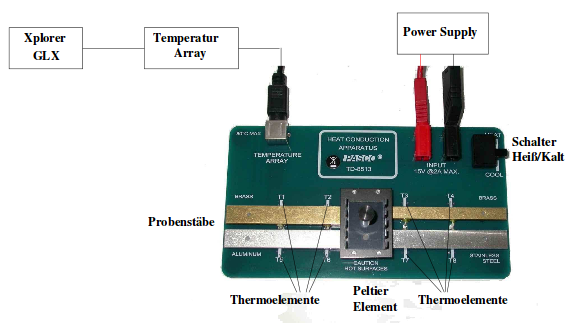
\includegraphics[width=\textwidth ]{Diagramme/v204aufbau.png}
\caption{Skizze zum Versuchsaufbau}
\label{aufbau}
\end{figure}
Zur Messung der Temparaturen der Metallstäbe ist ein Versuchsaufbau auf einer Grundplatte befestigt. Auf dieser Grundplatte sind vier Metallstäbe angebracht, an denen je zwei Thermoelemente in einem festgelegten Abstand befestigt sind. Ein Peltier-Element kann über seine Unterseite das eine Ende der Metallstäbe simultan erhitzen oder kühlen. Über ein Labornetzteil wird das Peltierelement mit Spannung versorgt, durch die Möglichkeit einer Umpolung kann das Peltier-Element entweder kühlen oder heizen. Die Temparaturen an den acht Thermoelementen werden von einem sogenannten Temparaturarray ausgelesen und per Datenkabel an einen Xplorer GLX \footnote{Kleincomputer zur Datenerfassung und Auswertung mit Druckfunktion für Tabellen und Graphen} gesendet.
In Absprache mit der Versuchsleitung wird zum Heizen der Metallstäbe eine Spannung von 8V angelegt und zur Kühlung eine Spannung von 5V. Aufgrund der geringen Effizienz des Peltierelementes würde dieses beim Kühlen warm werden und so die Kühlwirkung verschlechtern.
\subsection{Eigenschaften der Metallstäbe}
Über die vier Metallstäbe sind viele Eigenschaften bekannt. Sie werden in der folgenden Tabelle dargestellt:
\begin{table}[h]
\centering
\begin{tabular}{|c|c|c|c|c|}
\hline
Stoff & Abmessungen [cm] & $\rho \left[ \frac{kg}{m^3} \right] $ & $c \left[ \frac{J}{Kg \cdot K} \right]$ & $ \kappa_{Literatur}$ \\
\hline
Messing (schmal) & 9*0.7*0.4 & 8520 & 385 & ???\\
Messing (breit) & 9*1.2*0.4 & 8520 & 385 & ???\\
Aluminium (breit) & 9*1.2*0.4 & 2800 & 830 & ???\\
Edelstahl (breit) & 9*1.2*0.4 & 8000 & 400 & ???\\
\hline
\end{tabular}
\caption{Eigenschaften der Metallstäbe}
\end{table}
\subsection{Statische Methode}
In diesem Versuchsteil soll die Wärmeleitfähigkeit der verschiedenen Metalle ermittelt werden. Dazu werden die Metallstäbe dauerhaft erwärmt, bis der Edelstahl an Messpunkt T7 eine Temparatur von $45^\circ C$ besitzt. Alle fünf Sekunden werden die Temparaturen gemessen und in Abhändigkeit von der Zeit gespeichert. Zur Bestimmung des Metalles mit der besten Wärmeleitung werden die erreichten Temparaturen nach 700 Sekunden notiert. Nach erfolgreicher Messung werden die Metalstäbe aktiv gekühlt, bis sie eine Temparatur erreichen, die unter $30^\circ C$ liegt.
\subsection{Dynamische Methode}
Die dynamische Methode beruht auf dem Angström-Messverfahren. Bei diesem Messverfahren werden die Metallstäbe periodisch erwärmt und gekühlt. Dadurch bildet sich eine Temparaturwelle, die sich durch den Metallstab ausbreitet.
In den dynamischen Messungen werden die Temparaturen alle zwei Sekunden erfasst.
Es werden zwei Messreihen durchgeführt, die sich durch verschiedene Periodendauern unterscheiden. Es wird eine Messung mit einer Periodendauer von 80 sek und eine Messung mit einer Periodendauer von 200 sek durchgeführt. Zwischen den beiden Messreihen werden die Metallstäbe ausreichend gekühlt.

\section{Auswertung}
\subsection{Statische Methode}

Bei der ersten Messung wurden die Stäbe mit dem Peltierelement (Spannung $5V$) erhitzt und die Temperaturen an fernen Thermoelementen ($T_1, T_4, T_5, T_8$) gemessen.Die Abbildungen \ref{T1T4} und \ref{T5T8} zeigen diese Temperaturverläufe graphisch. Desweiteren ist zu erkennen, das die Temperaturen nach $700s$ folgende Werte habe.

\begin{tabular}{@{$\bullet$  }ll}
Messing &$T_1= 42.85 ^\circ C$\\
Messing &$T_4 =  40.69 ^\circ C$\\
Aluminum &$T_5 = 44.92 ^\circ C$\\
Edelstahl &$T_8 =33.17 ^\circ C$\\

\end{tabular}\\
Dieses Ergebnis zeigt qualitativ, dass Aluminum unter den untersuchten Materialien die höchste Wärmeleitfähigkeit besitzt.

\begin{figure}[H]
%
\includegraphics[angle=90, height=\textheight]{Diagramme/Abb1.eps}
\caption{Temperaturverläufe von zwei Messingstäben}
\label{T1T4}
\end{figure}

\begin{figure}[H]
\centering
%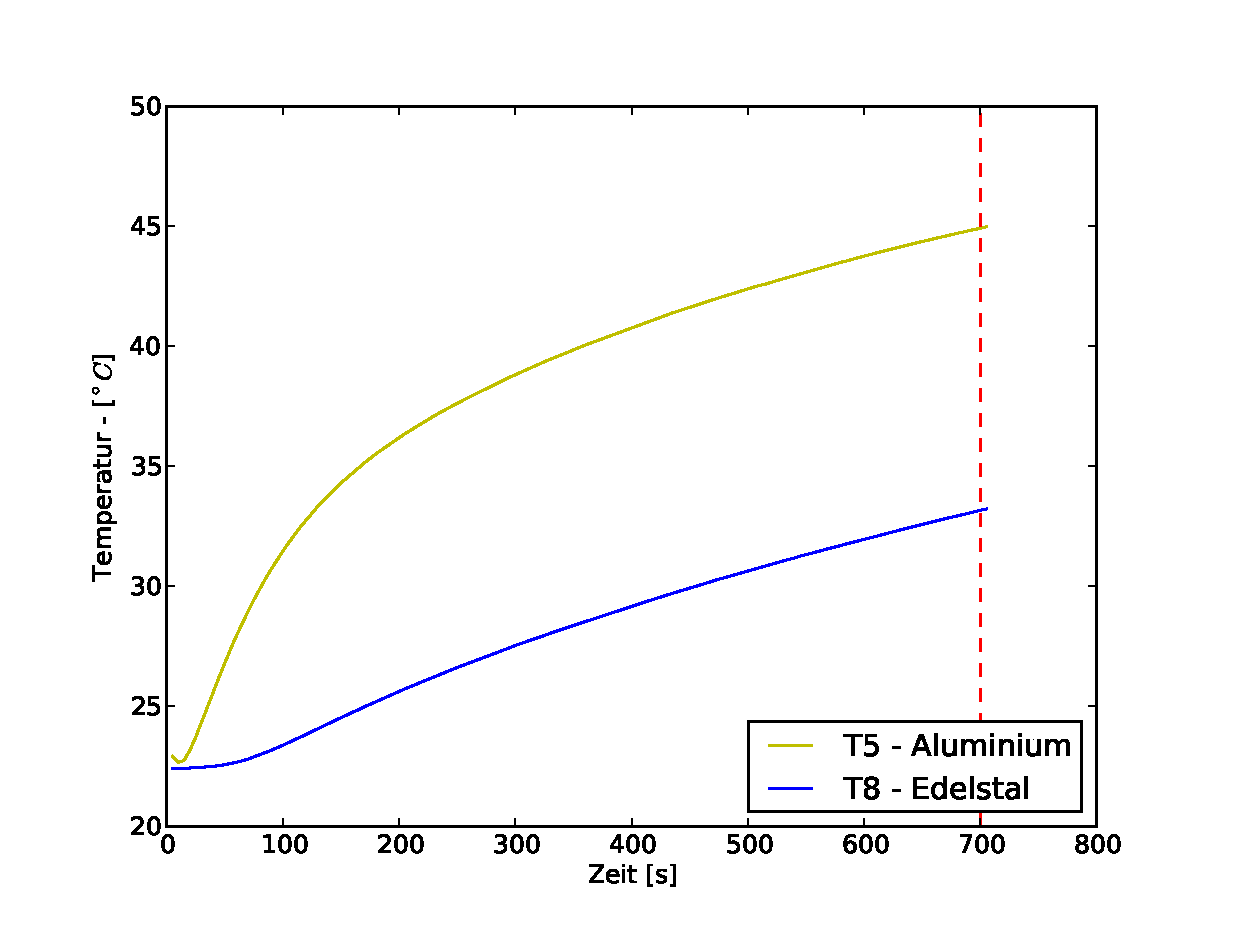
\includegraphics[angle=90,height=\textheight]{Diagramme/Abb2.eps}
\caption{Temperaturverläufe von zwei Messingstäben}
\label{T5T8}
\end{figure}
\section{Diskussion}
Hier kommt die Diskussion hin.
\section{Literatur- und Abbildungsverzeichnis}
Hier befindet sich das Literatur- und Abbildungsverzeichnis.
\section{Anhang}
Hier stehen die im Anhang angefügten Dokumente.
\end{document}
